\documentclass[dvipdfmx]{jsarticle}
\usepackage[T1]{fontenc}
\usepackage[dvipdfmx]{hyperref}
\usepackage{lmodern}
\usepackage{latexsym}
\usepackage{amsfonts}
\usepackage{amssymb}
\usepackage{mathtools}
\usepackage{nccmath}
\usepackage{amsthm}
\usepackage{multirow}
\usepackage[dvipdfmx]{graphicx}
\usepackage{wrapfig}
\usepackage{here}
\usepackage{float}
\usepackage{ascmac}
\usepackage{url}

\def\NO{04}
\def\LECTURENAME{論理と計算}
\begin{document}
\title{\LECTURENAME{}:第\NO{}回演習問題}

\author{5419045 高林秀}

\date{}
\maketitle

\begin{itemize}
\item Latexを用いて作成し,PDF形式で提出してください
\end{itemize}


\vspace*{\baselineskip}

\begin{enumerate}\setlength{\itemsep}{\baselineskip}

\item SAT問題とは何か,一言で端的に説明しなさい
\paragraph{解答}\par
モデルが存在するか否か(充足可能であるか否か)、すなわち命題論理式において、命題変数の真理値を定めることによって全体の論理式を真にできるかという問題。

\item SATとして定式化できる問題の具体例と,その問題におけるSAT符号化の指針を示しなさい
  (※「簡単に調査してください」ということです)
\paragraph{解答}\par
\begin{itemize}
  \item 具体例:数独問題
  \begin{figure}[H]
    \centering
    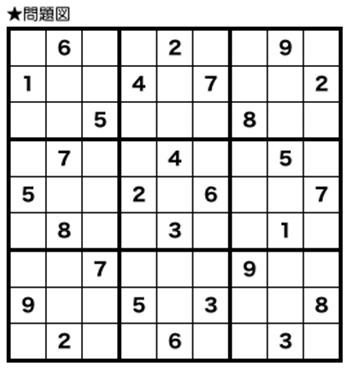
\includegraphics[scale=0.4]{sudoku.jpg}\par
    出典:\url{https://analytics-notty.tech/sudoku-rules/}
  \end{figure}
  \item SAT符号化の指針:以下のルールにおいて、順序符号化法と呼ばれる手法でSAT符号化する。\par
  1行1列のマスを$X_{1,1}$、1行2列のマスを$X_{1,2}$とする。このとき、$X_{1,1}$に$x^1,x^2, x^3,...x^8$、$X_{1,2}にx^{9}, x^{10}, ....,x^{16}$というように各マスに8個、合計で648個の命題変数を定める。
  \begin{itemize}
    \item 1つのマスに1〜9の数字が1つのみ入る。\par
    例えば、$X_{1,1}$について割り当てた8個の変数を使用して次の節ができる。
    \begin{align*}
      (\neg x^{1} \vee x^{2}) \wedge (\neg x^{2} \vee x^{3}) \wedge (\neg x^{3} \vee x^{4}) \wedge (\neg x^{4} \vee x^{5}) \wedge (\neg x^{5} \vee x^{6}) \wedge (\neg x^{6} \vee x^{7}) \wedge (\neg x_{7} \vee x_{8})
    \end{align*}
    この7節が各マスごとに存在するので、このルールは567節に符号化できる。\par
    以下下記のルールも同様に、Tseitin 変換と呼ばれる手法を使用してSAT符号化することができる。
    本稿では割愛する。
    \item 縦1列には1〜9の数字が1つずつ入る。\par
    \item 横1列には、1〜9の数字が1つずつ入る。
    \item $3\times 3$で囲まれた9マスには1〜9の数字が1つずつ入る。
  \end{itemize}
  \item 参考URL:\url{https://www.ipsj-kyushu.jp/page/ronbun/hinokuni/1002/C-5/C-5-4.pdf}
\end{itemize}


\item 節集合$\{(x_1\lor x_2), (\neg x_2 \lor \neg x_3\lor  \neg x_4), (x_1\lor x_4), (\neg x_2\lor x_3\lor \neg x_4)\}$の
  充足可能性判定を対象とした場合のDPLLの動作過程を示しなさい.
\paragraph{解答}




\item SATソルバーclaspを用い,以下の節集合に対する充足可能性を判定しなさい
(claspへの入力ファイルと実行方法,実行結果を示してください)

\[
\{(x_1\lor x_2), (\neg x_2 \lor \neg x_3\lor  \neg x_4), (x_1\lor x_4), (\neg x_2\lor x_3\lor \neg x_4)\}
\]
\paragraph{解答}\par
\begin{itemize}
  \item 入力ファイル q4.cnf
  \begin{verbatim}
    p cnf 4 4
    1 2 0
    -2 -3 -4 0
    1 4 0
    -2 3 -4 0
  \end{verbatim}
  \item 実行方法:\url{https://github.com/potassco/clasp/releases}よりバイナリファイルをダウンロードし、以下コマンドを実行する。
  \begin{verbatim}
    clasp-3.3.2/clasp-3.3.2-x86_64-linux 0 q4.cnf
  \end{verbatim}
  \item 実行結果
  \begin{verbatim}
    c clasp version 3.3.2
    c Reading from q4.cnf
    c Solving...
    c Answer: 1
    v 1 -2 -3 4 0
    c Answer: 2
    v 1 -2 -3 -4 0
    c Answer: 3
    v 1 -2 3 4 0
    c Answer: 4
    v 1 -2 3 -4 0
    c Answer: 5
    v 1 2 -3 -4 0
    c Answer: 6
    v 1 2 3 -4 0
    s SATISFIABLE
    c
    c Models         : 6
    c Calls          : 1
    c Time           : 0.000s (Solving: 0.00s 1st Model: 0.00s Unsat: 0.00s)
    c CPU Time       : 0.000s
  \end{verbatim}
  すなわち、$x_{1}, x_{4} = True、x_{2}, x_{3}=Falseのとき$、$x_{1} = True, x_{2}, x_{3}, x_{4} = Falseのとき$、$x_{1}, x_{3}, x_{4} = True、x_{2} = Falseのとき$、$x_{1}, x_{3} = True、x_{2}, x_{4} = Falseのとき$、$x_{1}, x_{2} = True、x_{3}, x_{4} = Falseのとき$、
  $x_{1}, x_{2}, x_{3} = True、x_{4} = False$のとき解釈は$True$になる。
  したがって充足可能である。
\end{itemize}


\item SATソルバーclaspを用い,以下の関係が成り立つことを示しなさい
(claspへの入力ファイルと実行方法,実行結果を示してください)
  \[
  \left\{ B_{11}\Leftrightarrow (P_{12}\lor P_{21}),~\neg B_{11}  \right\}
  \models
  \neg P_{12}\land \neg P_{21}
  \]

  ※SATソルバーへ入力できる形式に変形しましょう
  \paragraph{解答}
  \begin{itemize}
    \item 入力ファイル
    \begin{verbatim}
      p cnf 3 4
      -1 2 3 0
      1 -2 0
      1 -3 0
      -1 0
    \end{verbatim}
    \item 実行方法:以下のコマンドを入力する。
    \begin{verbatim}
         clasp-3.3.2/clasp-3.3.2-x86_64-linux 0 q5.cnf
    \end{verbatim}
    \item 結果
    \begin{verbatim}
      c clasp version 3.3.2
      c Reading from q5.cnf
      c Solving...
      c Answer: 1
      v -1 -2 -3 0
      s SATISFIABLE
      c
      c Models         : 1
      c Calls          : 1
      c Time           : 0.000s (Solving: 0.00s 1st Model: 0.00s Unsat: 0.00s)
      c CPU Time       : 0.000s
    \end{verbatim}
    したがって、$B_11 = False, P_12 = False, P_21 = False$のときに、節集合は充足可能である。このとき、$\neg p_12 \wedge \neg p_21$はTrueになるので成立する。
  \end{itemize}


\item 質問・コメント等がありましたらご記入ください(採点対象外です)

\end{enumerate}
\end{document}
